% Drawing 146/04-12 -- folder 146, batch 04, archive page 73 (PDF page 74).
% Transcription: Deux petites configurations de courbes stables, la première biffée.
% Kind: configurations of stable curves (schematic). Method 2 (schematic redraw from the facsimile). Status: ok.
% Notes: Left: a fan of three strokes, overinked (the struck configuration), drawn grey. Right: a horizontal component and a fan of three components from its right end. Whether the horizontal stroke belongs to the first or the second configuration cannot be decided from the page; drawn as it lies.
% Coordinates: 1 unit = 1 mm = 1/100 of the crop width (bbox in page fractions: [0.38, 0.64, 0.52, 0.73]).
% Redrawn by Claude (claude-opus-5-5), issue #73 pilot, 2026-11-07; not checked by a human; not compiled (no TeX in the session).
% Rights: reproduces part of the work -- behind RENDER_TRANSCRIPTS, never published by itself.
\documentclass[tikz,border=3pt]{standalone}
\usepackage{amsmath,amssymb}
\usetikzlibrary{patterns,arrows.meta}
\tikzset{pencil/.style={black!45}, struck/.style={black!35}, mark/.style={circle,draw,inner sep=1.3pt}, pt/.style={circle,fill,inner sep=0.9pt}, opt/.style={circle,draw,fill=white,inner sep=1.1pt}}
\begin{document}
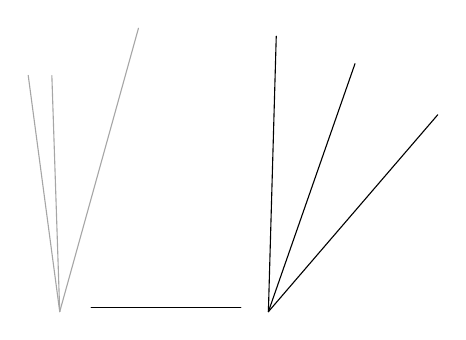
\begin{tikzpicture}[x=1mm,y=1mm,line cap=round,line join=round,font=\scriptsize]
\draw[struck] (25,-61) -- (21,-31);
\draw[struck] (25,-61) -- (24,-31);
\draw[struck] (25,-61) -- (35,-25);
\draw (29,-60.5) -- (48,-60.5);
\draw (51.5,-61) -- (52.5,-26);
\draw (51.5,-61) -- (62.5,-29.5);
\draw (51.5,-61) -- (73,-36);
\end{tikzpicture}
\end{document}
